\documentclass[a4paper,12pt]{article}
\usepackage[T1,T2A]{fontenc}
\usepackage[utf8]{inputenc}
\usepackage[english,ukrainian]{babel}


\usepackage{ upgreek }
\usepackage{amsmath}

\DeclareMathOperator*{\argmax}{arg\,max}
\DeclareMathOperator*{\argmin}{arg\,min}

\usepackage{graphicx}
\graphicspath{{./pictures/}}


\usepackage[unicode=true,colorlinks=true,urlcolor=blue,citecolor=green,linkcolor=blue]{hyperref}
\usepackage[ukrainian,nameinlink]{cleveref}
\usepackage{geometry} % Меняем поля страницы
\geometry{left=2cm}% левое поле
\geometry{right=1.5cm}% правое поле
\geometry{top=1cm}% верхнее поле
\geometry{bottom=2cm}% нижнее поле



\begin{document}
	
	\begin{titlepage}
		\vspace*{6cm}
		\begin{center}
			
			\large
			\textbf{Звіт}\\
			\textbf{до лабораторної роботи №5:}\\
			\textbf{<<Метод $k$-середніх>>}
			
		\end{center}
		
		\vspace{8cm}
		\begin{flushright}
			студента 1-го курсу магістратури\\
			факультету комп'ютерних наук та кібернетики\\
			Кравця Олексія
		\end{flushright}
		
	\end{titlepage}

\newpage
\tableofcontents
\newpage
%document here
\section{Постановка задачі}
	Використовуючи метод $k$-середніх необхідно провести кластерізацію точок на площині. Візуалізувати результати використовуючи діаграму Вороного.
\section{Метод $k$-середніх}

\textbf{Метод $k$-середніх} -- популярний метод кластерізації. Алгоритм намагається мінімізувати сумарне квадратичне відхилення точок кластерів від центрів цих кластерів:

\[
	V = \sum_{i=1}^{k}\sum_{x \in S_i} (x - \mu_i)^2
\]
де $k$ -- число кластерів, $S_i$ -- отримані кластери, $i = 1,2,\ldots, j$, а $\mu_i$ -- центри мас всіх векторів $x$ з кластера $S_i$.

Головна ідея алгоритму полягає у перерахуванні на кожній ітерації центрів мас всіх кластерів, що були отримані на минулій ітерації. Після цього вектори знову розбиваються на кластери відповідно до отриманих центрів мас.

Алгоритм завершується, коли на деякій ітерації не змінюються центри кластерів. Це досягається за скінченну кількість кроків.

\section{Результати}

Сгенеруємо набір точок на площині, що після цього будемо кластерізувати на 4 класи.  Сгенеруємо точки з такими розподілами:

\begin{itemize}
	\item Нормальний розподіл. По осі $x$ маємо $\mu = 3, \sigma = 0.2$, по осі $y$ маємо $\mu = 5, \sigma = 0.2$ 
	\item Нормальний розподіл. По осі $x$ маємо $\mu = 1, \sigma = 0.1$, по осі $y$ маємо $\mu = 1, \sigma = 0.7$ 
	\item Нормальний розподіл. По осі $x$ маємо $\mu = 5, \sigma = 1$, по осі $y$ маємо $\mu = 2, \sigma = 0.01$  
	\item Нормальний розподіл. По осі $x$ маємо $\mu = 5, \sigma = 0.01$, по осі $y$ маємо $\mu = 1, \sigma = 0.01$
\end{itemize}

Оберемо початкові центри кластерів:
\[
	\mu_0 = (3,4) \quad \mu_1 = (2,1) \\
	\mu_2 = (5,4) \quad \mu_3 = (4,1)
\]

На рисунку \ref{fig:1} можна побачити точки, що будемо кластерізувати (чорні точки), початкове наближення для центрів кластерів. Також на рисунку \ref{fig:1} зображено діаграму Вороного.

\newpage
\begin{figure}[h]
	\center{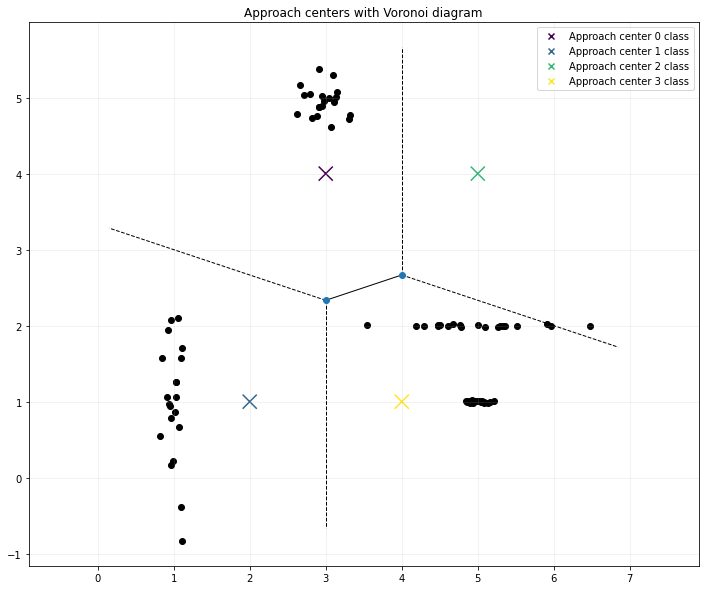
\includegraphics[scale=0.7]{fig1.png}}
	\caption{Точки для кластерізації}
	\label{fig:1}
\end{figure}

Давайте поглянемо на вигляд методу після однієї ітерації. На рисунку \ref{fig:2} зображено результат \textbf{методу $k$-середніх} після 1 ітерації. Розглянемо відстань на яку змістилися центри кластерів:

\begin{itemize}
	\item Центр кластеру $0$ змістився на $0.95$
	\item Центр кластеру $1$ змістився на $1$
	\item Центр кластеру $2$ змістився на $2.49$
	\item Центр кластеру $3$ змістився на $1.06$	
\end{itemize}

\newpage
\begin{figure}[h]
	\center{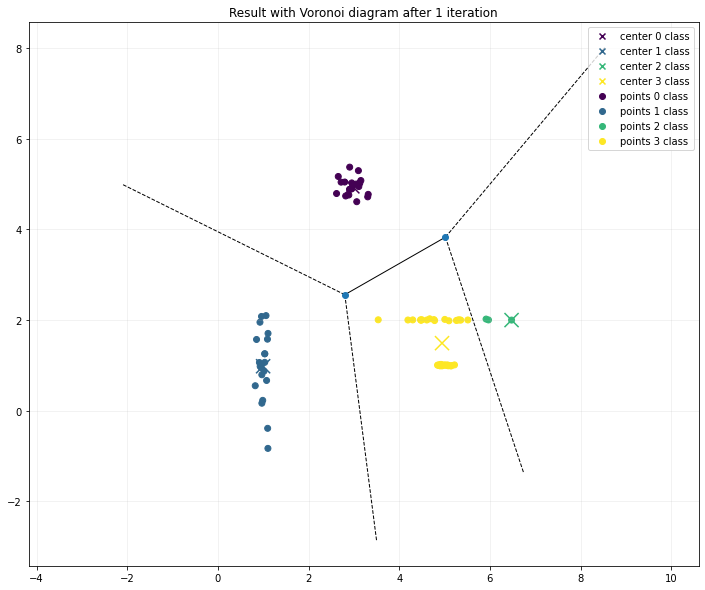
\includegraphics[scale=0.7]{fig2.png}}
	\caption{Після 1 ітерації}
	\label{fig:2}
\end{figure}

Тепер запустимо алгоритм, доки не отримаємо ітерацію для якої, максимальне зміщення центрів кластерів буде менше $10^{-5}$. Виведемо результат на рисунку \ref{fig:3}.

\newpage
\begin{figure}[h]
	\center{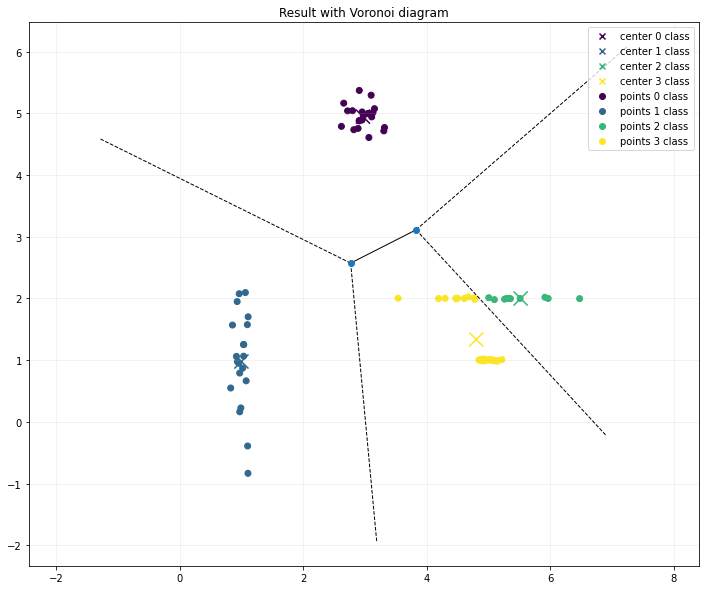
\includegraphics[scale=0.7]{fig3.png}}
	\caption{Результат}
	\label{fig:3}
\end{figure}

\section{Висновки}

Метод $k$-середніх спрацював на тестових даних коректно та розділив точки на $4$ класи. Але метод не зміг знайти кластери, що відповідали б заданим нормальним розподілам точок. Про це свідчить неточне розділення точок на \textbf{2} та \textbf{3} кластери. Можливо більш точний підбір початкових центрів кластерів може вирішити цю проблему.

\end{document}
